\chapter{Diseño}

\section{Requerimientos}
Antes de empezar con el desarrollo de nuestro proyecto, debemos definir la funcionalidad del mismo explicando detalladamente como sería el comportamiento de cada una de las partes implicadas.

\begin{itemize}
\item \textbf{Web}: Creación de una interfaz con la que poder interaccionar con las preguntas del bot y mensajes a mostar.
\begin{itemize}
\item Implementación de un login y un registro para que solo los usuarios registrados puedan acceder al panel de control.
\item Panel de control, primera vista del usuario que funciona como guía para las operaciones a realizar.
\item Apartado de preguntas, bloques, preámbulos, respuestas y gestión de usuarios.
\item Vistas de detalle y operaciones de modificación, clonado y borrado de cada uno de los apartados anteriores.
\item Autenticación y permisos en la realización de operaciones solo para usuarios específicos.
\item Descarga de las respuestas proporcionadas por los usuarios en formato CSV.

\end{itemize}

\item \textbf{Chatbot}: Creación de un chatbot en línea que realice un cuestionario de preguntas y a su vez una lógica interna que permita una interacción con el usuario.
\begin{itemize}
\item Mensaje de bienvenida al usuario cuando entre en el chat del bot.
\item Almacenamiento del usuario como un nuevo integrante de nuestro sistema si ningún tipo de cuestionario gracias a las funciones especificas de Telegram que permiten la obtención de los datos del usuario que se encuentra activo en el chat.
\item Entorno de interacción por parte del bot con el usuario para poder tener una conversación lo más humana posible mediante el análisis de ciertas palabras e ideas previamente establecidas.
\item Cuestionario de preguntas que se encuentran activas para los usuarios en un momento concreto. Estas preguntas varían dependiendo de la planificación de los cuestionarios y la frecuencia de cada uno de ellos.
\item Recolección y almacenamiento de las respuestas proporcionadas en la base de datos de forma automática.
\item Creación de avisos a todos los usuarios cuando haya cuestionarios pendientes, dependiendo de la hora y frecuencia de cada uno de ellos.
\item Realización de este proceso de forma cíclica sin que el usuario pierda el hilo conductor de la conversación y además que cada proceso sea totalmente independiente para cada usuario.
\end{itemize}
\end{itemize}

\section{Arquitectura}

El objetivo del proyecto es conseguir información estructurada a partir de las experiencias y emociones de los usuarios. Con este objetivo se ha diseñado una arquitectura que consta de tres componentes principales: aplicación web, chatbot y base de datos. La aplicación web actúa como panel de control para que el administrador tenga acceso a la gestión de los cuestionarios, el chatbot se encarga de interactuar con los usuarios realizando preguntas con el objetivo de obtener respuestas. Por último la base de datos que almacena que almacena los datos relevantes y permite un fácil acceso a esta información. Gracias a esto se consigue una solución integral que combina la facilidad de uso del chatbot en Telegram con la capacidad de gestión y análisis dada por la aplicación web.

En la \textit{\hyperref[fig:arquitectura]{Figura 4.2}}, se presenta de manera detallada la arquitectura que hemos empleado en nuestro proyecto. Esta representación gráfica es fundamental para comprender la estructura subyacente de nuestro sistema y cómo se interconectan sus diversos componentes. A través de esta figura, se destila una visión completa de la disposición y relación de los elementos clave que conforman nuestra solución.

\clearpage

\begin{sidewaysfigure}[!ht]
    \centering
    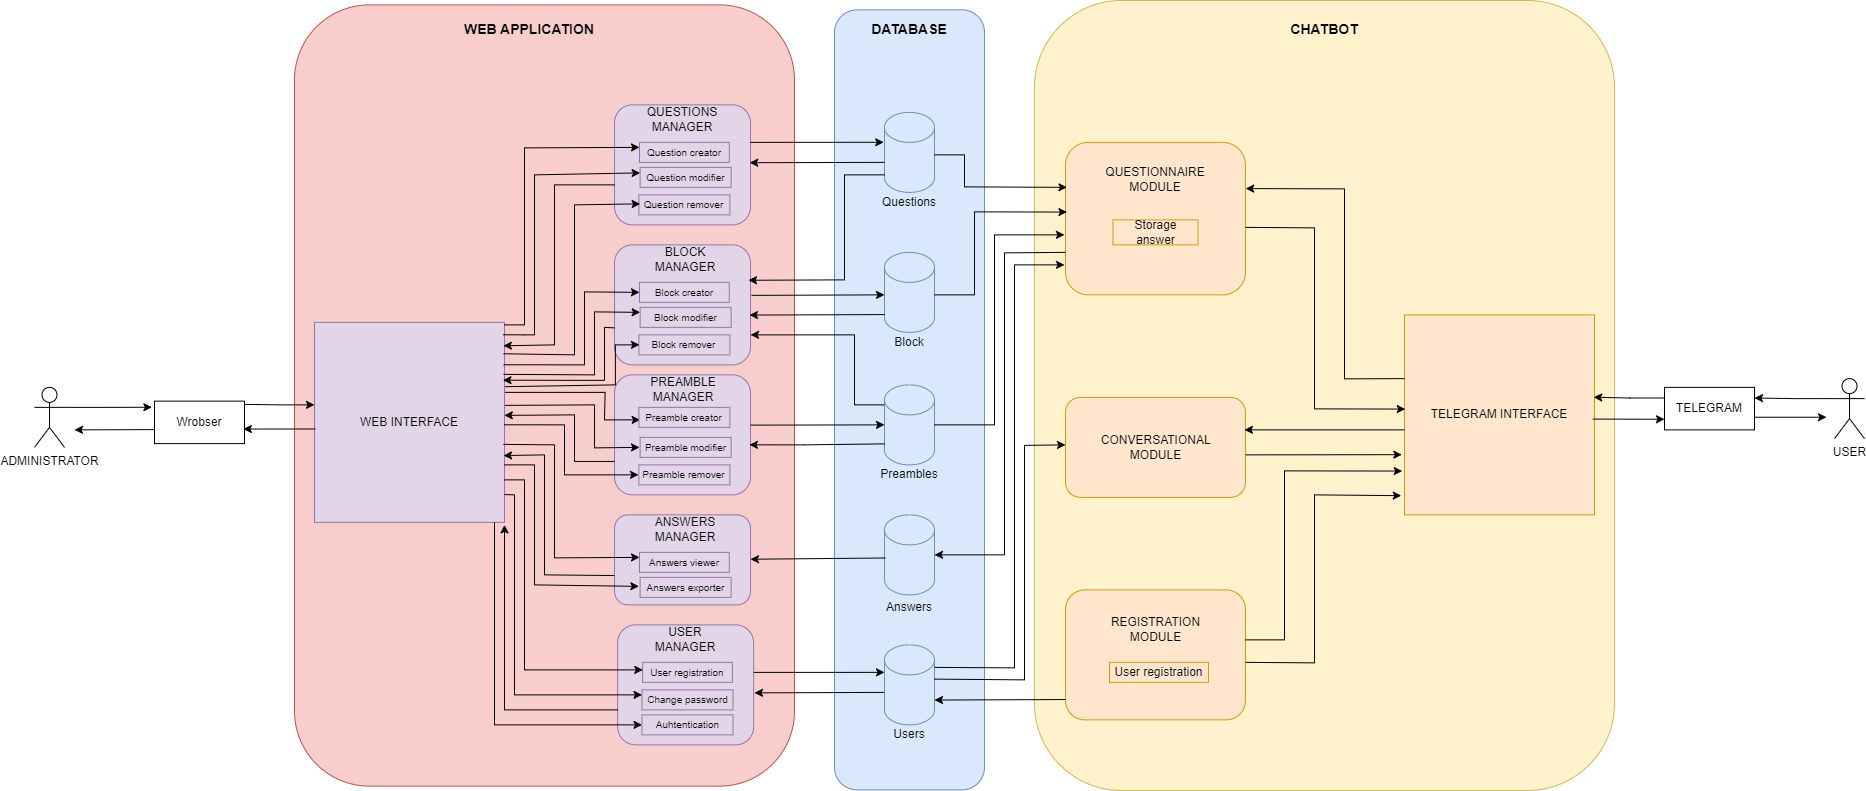
\includegraphics[width=1\textheight]{imagenes/Arquitecture2.drawio.png}
    \caption{\textit{POSTCOVID-AI TELEGRAMBOT} arquitectura}
    \label{fig:arquitectura}
\end{sidewaysfigure}
\clearpage

\begin{comment}
En la \textit{\hyperref[fig:diagrama]{figura 4.1}} vemos el diagrama de clases que muestra las relaciones entre las entidades existentes en el sistema. Esta base de datos consta de cinco entidades principales:
\begin{itemize}
\item \textbf{Peguntas}: Contiene la información de todas las preguntas almacenadas. Esta se divide en dos: Pregunta y Posibles respuestas. Dentro de la primera especificaría el título de la pregunta junto con otros campos como la fecha o usuario de creación y la segunda contiene las respuestas a esa pregunta. 
\item \textbf{Bloques de Preguntas}: Las preguntas se estructuran en bloques. Cada bloque puede tener las preguntas que desee, junto a otros atributos para que permiten su planificación. Los bloques también tienen asociado un preámbulo. 
\item \textbf{Preámbulos}: Dentro de los preámbulos se guardan los mensajes a mostrar por el bot cuando se hable de un tema concreto. Si un bloque tiene asociado un preámbulo, en el momento que se realice el cuestionario asociado a ese bloque de preguntas el bot mostrará cualquiera de los mensajes de ese preámbulo de forma aleatoria. De esta forma nos aseguramos la interactividad y que la experiencia sea diferente para cada usuario.
\item \textbf{Usuarios}: Guarda los agentes registrados en nuestro sistema. Se divide en dos tipos: los administradores que tienen acceso al panel de control y los usuarios comúnes que son los que interactúan con el bot.
\item \textbf{Respuestas}: Contiene las respuestas de los usuarios a las preguntas. Solo se almacenan las respuestas posibles de cada pregunta para así confirmar que la información sea correcta.
\end{itemize}

\begin{figure}[!ht]
    \centering
    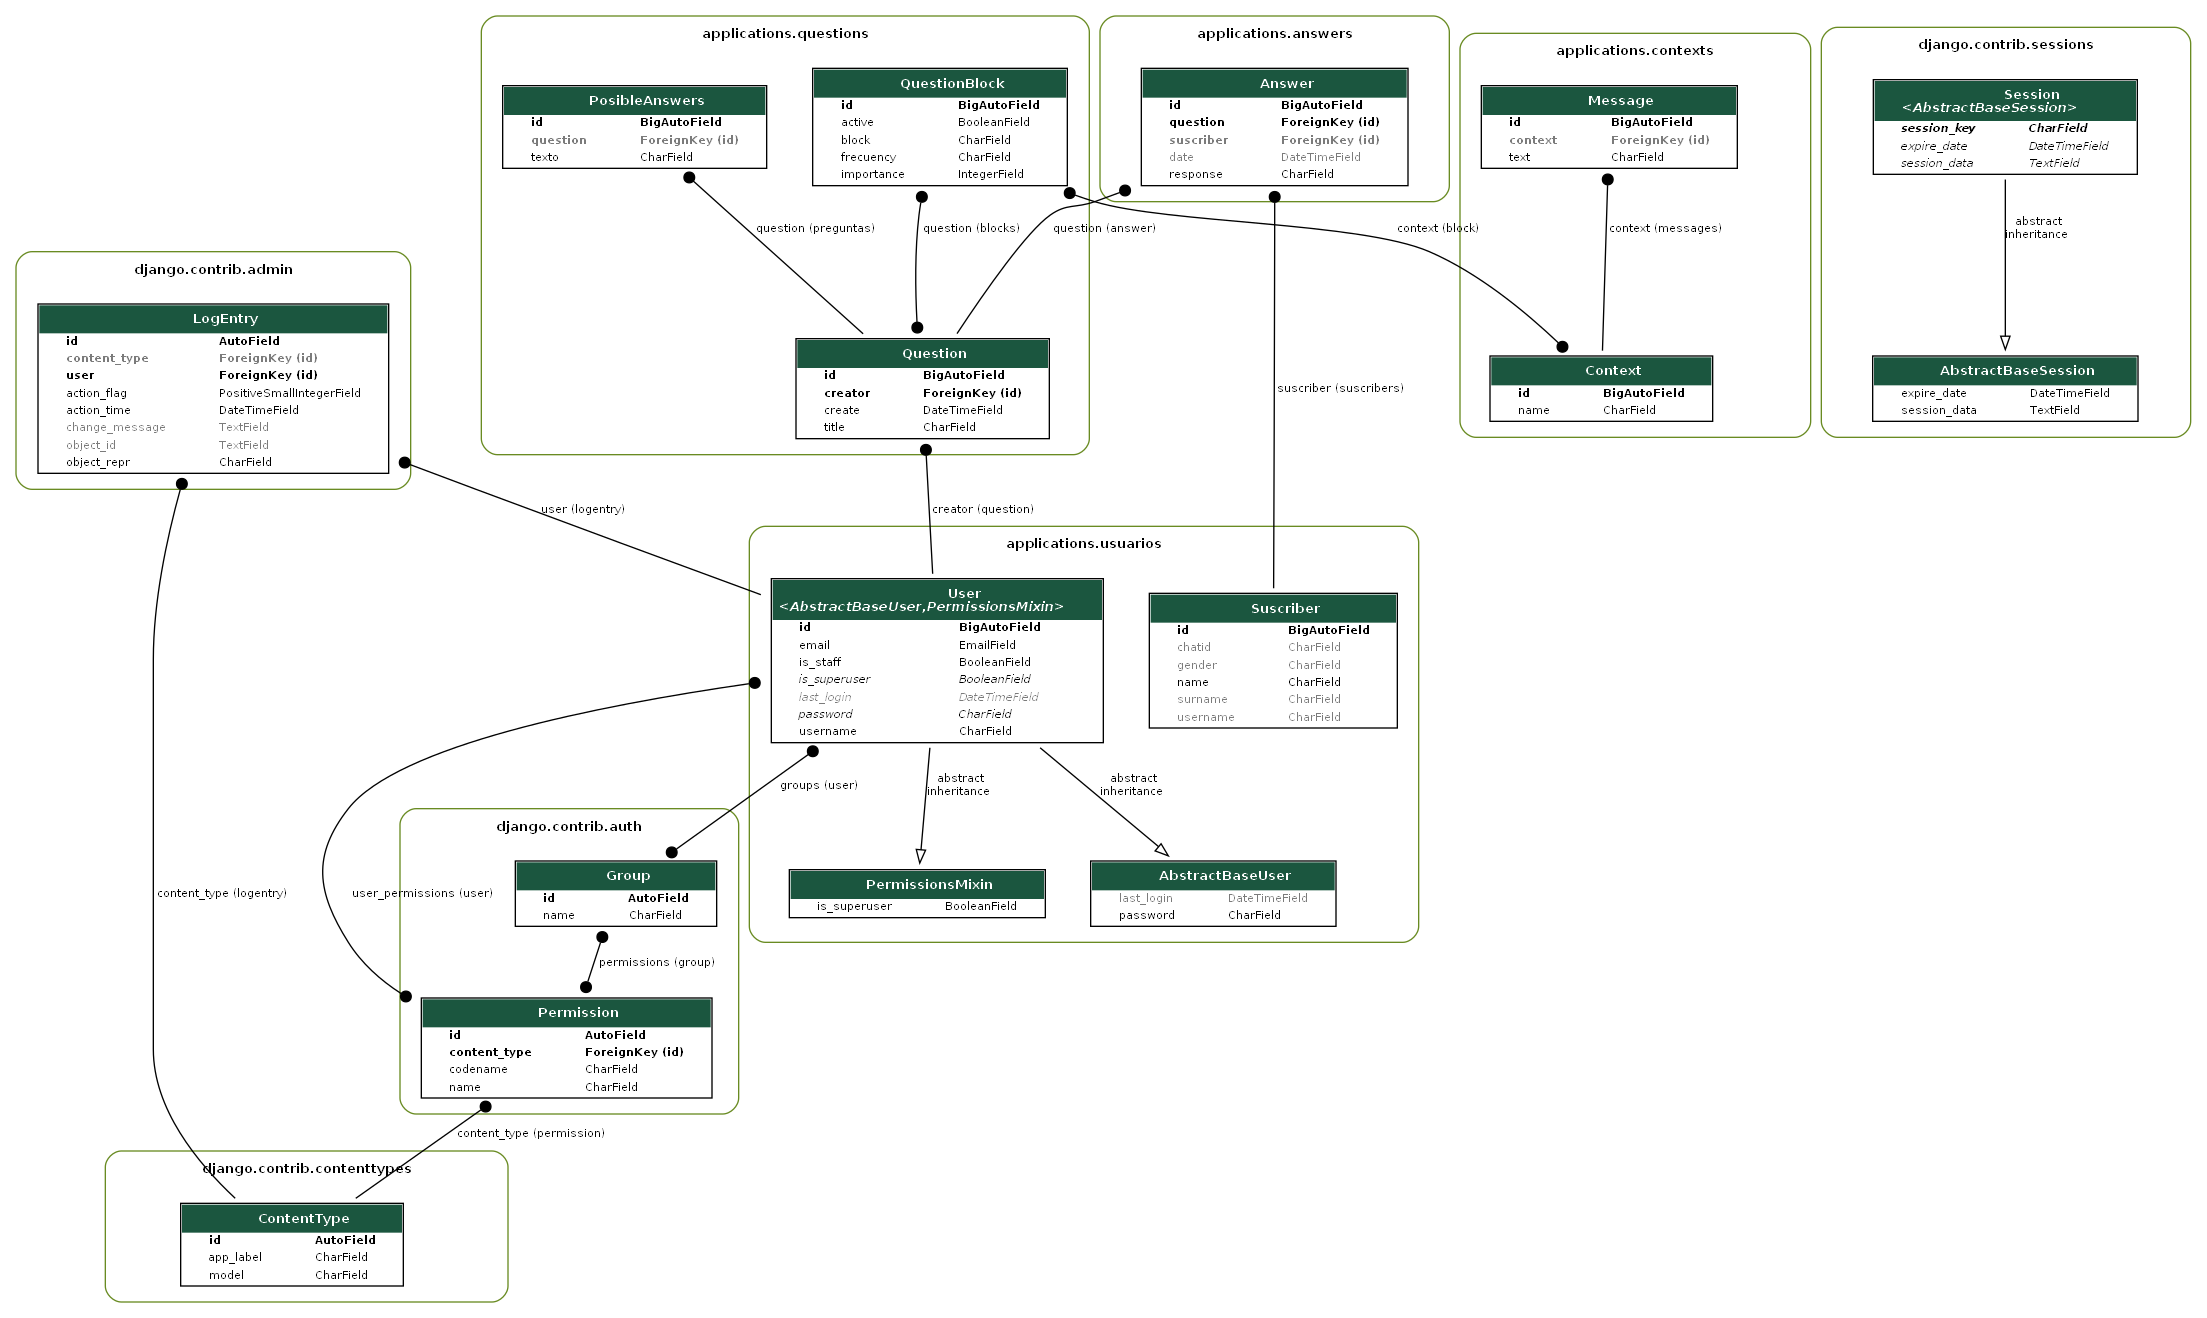
\includegraphics[width=1\textwidth, height=15cm]{imagenes/myapp_models.png}
    \caption{ Diagrama de clases }
    \label{fig:diagrama}
\end{figure}

\end{comment}

La base de datos se encuentra estructurada en cinco modelos: preguntas, preámbulos, bloques, respuestas y usuarios. Posteriormente se analizarán con más detalle.

La aplicación web esta formada por cinco módulos. El primero es el question manager, que permite la creación, modificación y borrado de preguntas. Seguido del preamble manager, el cual tiene la misma funcionalidad que el anterior pero con los preámbulos. Después se encuentra el block manager, que también consta con las operaciones básicas para la gestión de los bloques. Tanto las preguntas como los preámbulos interactúan con este módulo. En cuarto lugar se encuentra el answer manager, que guarda las respuestas obtenidas por los usuarios e interactúa con el último módulo. User manager, contiene la información de los usuarios registrados en nuestro sistema.

La parte del chatbot está formada por tres módulos. Un primer módulo de bienvenida y registro, donde el bot se presenta al usuario y lo guarda como un nuevo registro en la base de datos. Un segundo módulo que actúa como agente conversacional. Y por último, un tercer módulo que representa el cuestionario de preguntas. Este módulo interactúa con las preguntas, bloques y preámbulos creados a través de la aplicación web. Recoge las respuestas de los usuarios y las guarda en la base de datos.

Esta arquitectura permite la creación, gestión y control de cuestionarios interactivos, mensajes generados, administración de usuarios a través de la aplicación web y la recogida y clasificación de respuestas. 








